% Source: tex/chapters/ch06/04_ソフトウェアエンジニアリング運用の基礎.tex
\subsubsection{ソフトウェアエンジニアリング運用プロセス}

運用プロセスは、既存のソフトウェアシステムまたは製品を配備、設定、運用、支援し、その完全性を保つための活動である。国際標準では、運用の準備、運用の実行、運用結果の管理、利用者支援が重要な活動として扱われる。

SWEBOK 06章では、運用活動を学習しやすくするため、次の三つのプロセス群として整理できる。

\par\smallskip\noindent\refstepcounter{table}\label{tab:ch06-03}\textbf{表 \thetable: 第06章 ソフトウェアエンジニアリング運用 表03}\par\smallskip
\begin{longtable}{L{35mm}L{115mm}}
\toprule
プロセス群 & 含まれる活動 \\
\midrule
運用計画 & 運用計画、供給者管理、開発環境と運用環境、可用性、継続性、サービス水準、容量、バックアップ、災害復旧、フェイルオーバー、安全性とセキュリティを扱う。 \\
運用提供 & 運用テスト、検証、受け入れ、配備、リリース、ロールバック、データ移行、問題解決を扱う。 \\
運用制御 & インシデント管理、変更管理、監視、測定、追跡、レビュー、運用支援、サービス報告を扱う。 \\
\bottomrule
\end{longtable}

\begin{figure}[htbp]
\centering
\IfFileExists{assets/generated_figures/ch06/fig-ch06-02.png}{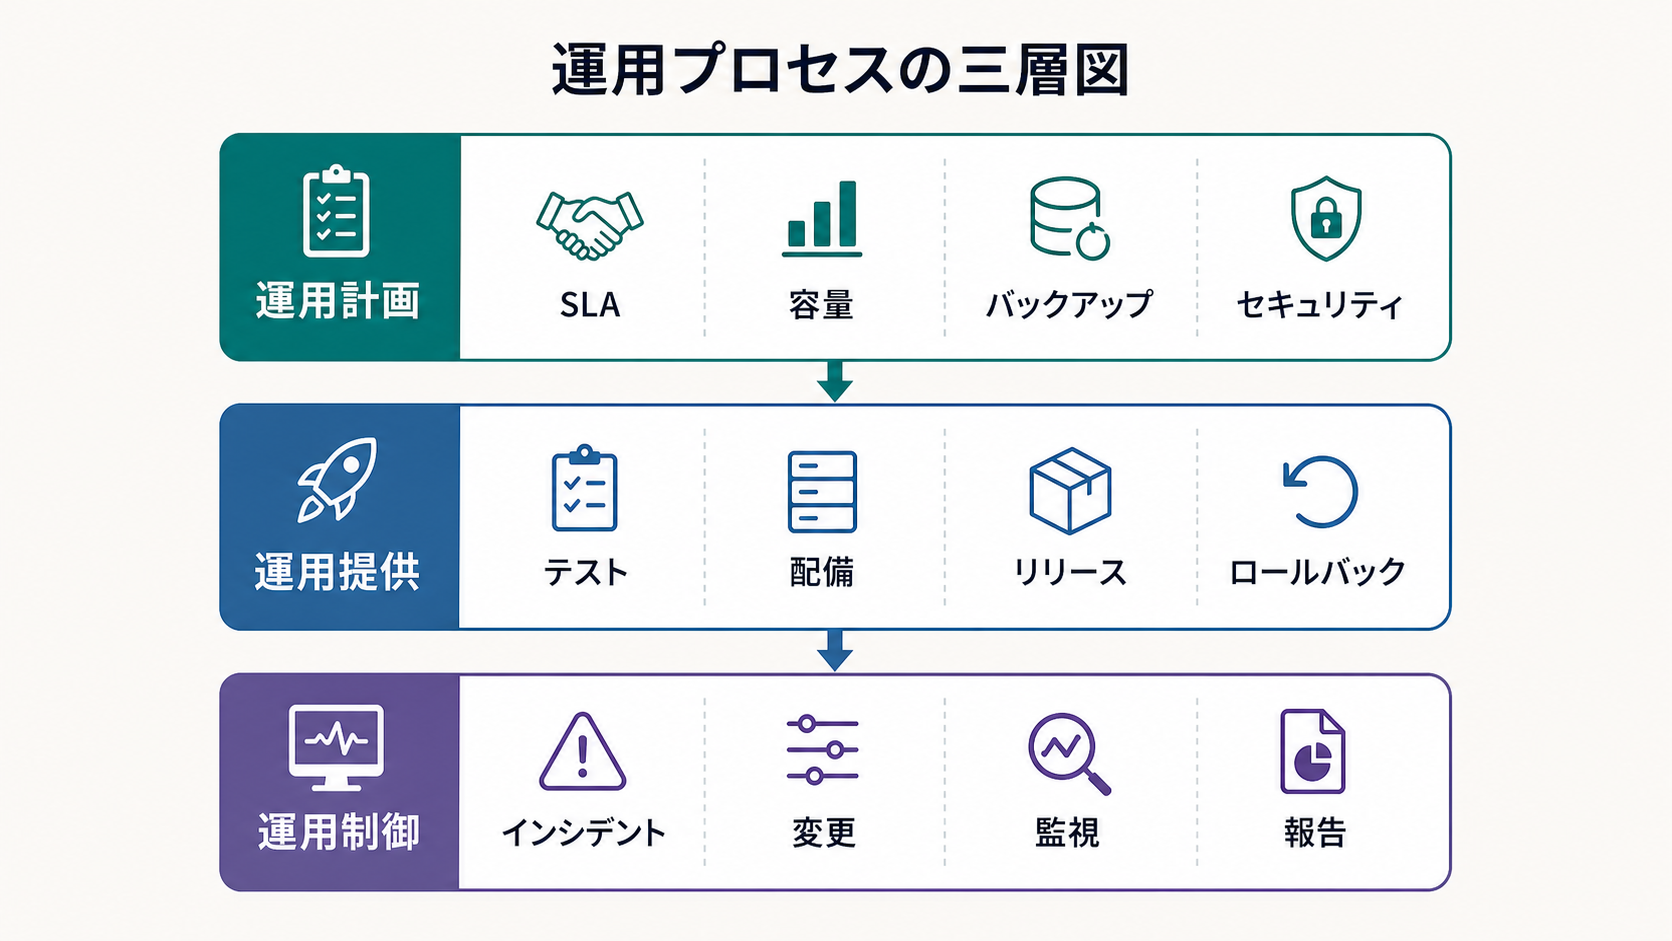
\includegraphics[width=0.96\linewidth]{assets/generated_figures/ch06/fig-ch06-02.png}}{\fbox{\parbox[c][48mm][c]{0.9\linewidth}{\centering 画像生成待ち\\運用プロセスの三層図}}}
\caption{運用プロセスの三層図}
\label{fig:ch06-02}
\end{figure}
